% Options for packages loaded elsewhere
\PassOptionsToPackage{unicode}{hyperref}
\PassOptionsToPackage{hyphens}{url}
%
\documentclass[
]{article}
\usepackage{lmodern}
\usepackage{amssymb,amsmath}
\usepackage{ifxetex,ifluatex}
\ifnum 0\ifxetex 1\fi\ifluatex 1\fi=0 % if pdftex
  \usepackage[T1]{fontenc}
  \usepackage[utf8]{inputenc}
  \usepackage{textcomp} % provide euro and other symbols
\else % if luatex or xetex
  \usepackage{unicode-math}
  \defaultfontfeatures{Scale=MatchLowercase}
  \defaultfontfeatures[\rmfamily]{Ligatures=TeX,Scale=1}
\fi
% Use upquote if available, for straight quotes in verbatim environments
\IfFileExists{upquote.sty}{\usepackage{upquote}}{}
\IfFileExists{microtype.sty}{% use microtype if available
  \usepackage[]{microtype}
  \UseMicrotypeSet[protrusion]{basicmath} % disable protrusion for tt fonts
}{}
\makeatletter
\@ifundefined{KOMAClassName}{% if non-KOMA class
  \IfFileExists{parskip.sty}{%
    \usepackage{parskip}
  }{% else
    \setlength{\parindent}{0pt}
    \setlength{\parskip}{6pt plus 2pt minus 1pt}}
}{% if KOMA class
  \KOMAoptions{parskip=half}}
\makeatother
\usepackage{xcolor}
\IfFileExists{xurl.sty}{\usepackage{xurl}}{} % add URL line breaks if available
\IfFileExists{bookmark.sty}{\usepackage{bookmark}}{\usepackage{hyperref}}
\hypersetup{
  pdftitle={Project 2},
  hidelinks,
  pdfcreator={LaTeX via pandoc}}
\urlstyle{same} % disable monospaced font for URLs
\usepackage[margin=1in]{geometry}
\usepackage{color}
\usepackage{fancyvrb}
\newcommand{\VerbBar}{|}
\newcommand{\VERB}{\Verb[commandchars=\\\{\}]}
\DefineVerbatimEnvironment{Highlighting}{Verbatim}{commandchars=\\\{\}}
% Add ',fontsize=\small' for more characters per line
\usepackage{framed}
\definecolor{shadecolor}{RGB}{248,248,248}
\newenvironment{Shaded}{\begin{snugshade}}{\end{snugshade}}
\newcommand{\AlertTok}[1]{\textcolor[rgb]{0.94,0.16,0.16}{#1}}
\newcommand{\AnnotationTok}[1]{\textcolor[rgb]{0.56,0.35,0.01}{\textbf{\textit{#1}}}}
\newcommand{\AttributeTok}[1]{\textcolor[rgb]{0.77,0.63,0.00}{#1}}
\newcommand{\BaseNTok}[1]{\textcolor[rgb]{0.00,0.00,0.81}{#1}}
\newcommand{\BuiltInTok}[1]{#1}
\newcommand{\CharTok}[1]{\textcolor[rgb]{0.31,0.60,0.02}{#1}}
\newcommand{\CommentTok}[1]{\textcolor[rgb]{0.56,0.35,0.01}{\textit{#1}}}
\newcommand{\CommentVarTok}[1]{\textcolor[rgb]{0.56,0.35,0.01}{\textbf{\textit{#1}}}}
\newcommand{\ConstantTok}[1]{\textcolor[rgb]{0.00,0.00,0.00}{#1}}
\newcommand{\ControlFlowTok}[1]{\textcolor[rgb]{0.13,0.29,0.53}{\textbf{#1}}}
\newcommand{\DataTypeTok}[1]{\textcolor[rgb]{0.13,0.29,0.53}{#1}}
\newcommand{\DecValTok}[1]{\textcolor[rgb]{0.00,0.00,0.81}{#1}}
\newcommand{\DocumentationTok}[1]{\textcolor[rgb]{0.56,0.35,0.01}{\textbf{\textit{#1}}}}
\newcommand{\ErrorTok}[1]{\textcolor[rgb]{0.64,0.00,0.00}{\textbf{#1}}}
\newcommand{\ExtensionTok}[1]{#1}
\newcommand{\FloatTok}[1]{\textcolor[rgb]{0.00,0.00,0.81}{#1}}
\newcommand{\FunctionTok}[1]{\textcolor[rgb]{0.00,0.00,0.00}{#1}}
\newcommand{\ImportTok}[1]{#1}
\newcommand{\InformationTok}[1]{\textcolor[rgb]{0.56,0.35,0.01}{\textbf{\textit{#1}}}}
\newcommand{\KeywordTok}[1]{\textcolor[rgb]{0.13,0.29,0.53}{\textbf{#1}}}
\newcommand{\NormalTok}[1]{#1}
\newcommand{\OperatorTok}[1]{\textcolor[rgb]{0.81,0.36,0.00}{\textbf{#1}}}
\newcommand{\OtherTok}[1]{\textcolor[rgb]{0.56,0.35,0.01}{#1}}
\newcommand{\PreprocessorTok}[1]{\textcolor[rgb]{0.56,0.35,0.01}{\textit{#1}}}
\newcommand{\RegionMarkerTok}[1]{#1}
\newcommand{\SpecialCharTok}[1]{\textcolor[rgb]{0.00,0.00,0.00}{#1}}
\newcommand{\SpecialStringTok}[1]{\textcolor[rgb]{0.31,0.60,0.02}{#1}}
\newcommand{\StringTok}[1]{\textcolor[rgb]{0.31,0.60,0.02}{#1}}
\newcommand{\VariableTok}[1]{\textcolor[rgb]{0.00,0.00,0.00}{#1}}
\newcommand{\VerbatimStringTok}[1]{\textcolor[rgb]{0.31,0.60,0.02}{#1}}
\newcommand{\WarningTok}[1]{\textcolor[rgb]{0.56,0.35,0.01}{\textbf{\textit{#1}}}}
\usepackage{graphicx,grffile}
\makeatletter
\def\maxwidth{\ifdim\Gin@nat@width>\linewidth\linewidth\else\Gin@nat@width\fi}
\def\maxheight{\ifdim\Gin@nat@height>\textheight\textheight\else\Gin@nat@height\fi}
\makeatother
% Scale images if necessary, so that they will not overflow the page
% margins by default, and it is still possible to overwrite the defaults
% using explicit options in \includegraphics[width, height, ...]{}
\setkeys{Gin}{width=\maxwidth,height=\maxheight,keepaspectratio}
% Set default figure placement to htbp
\makeatletter
\def\fps@figure{htbp}
\makeatother
\setlength{\emergencystretch}{3em} % prevent overfull lines
\providecommand{\tightlist}{%
  \setlength{\itemsep}{0pt}\setlength{\parskip}{0pt}}
\setcounter{secnumdepth}{-\maxdimen} % remove section numbering

\title{Project 2}
\author{}
\date{\vspace{-2.5em}}

\begin{document}
\maketitle

\emph{The dataset I used for my project was the Beat the Blues (BtheB)
dataset. It is a longitudinal study from a clinical trial that contains
data on the effects of a multimedia program ``Beat the Blues'', that
serves as cognitive therapy, on depression levels of depressed patients.
The dataset has 100 observations and 8 variables. The first variable is
a catergorical variable that specfies whether or not the patient took
anti-depressent drugs. The next variable is length which indicates
whether the current episode of depression has lasted more than or less
than six months. Treatment group is the last catergorical variable and
states whether the patient recieved the Beat the Blues treatment or
thier usual treatment. The rest of the variables which includes bdi.pre,
bdi.2m, bdi.4m, bdi.6m, bdi.8m are all numeric. They indicate the Beck
Depression Inventory II score before, 2 months, 4 months, 6 months, and
8 months after the treatment respectively. }

\begin{Shaded}
\begin{Highlighting}[]
\KeywordTok{options}\NormalTok{(}\DataTypeTok{repos=}\StringTok{"https://cran.rstudio.com"}\NormalTok{ )}

\KeywordTok{install.packages}\NormalTok{(}\StringTok{"HSAUR"}\NormalTok{,}\DataTypeTok{repos=}\StringTok{"https://cran.rstudio.com"}\NormalTok{)}
\end{Highlighting}
\end{Shaded}

\begin{verbatim}
## package 'HSAUR' successfully unpacked and MD5 sums
checked
##
## The downloaded binary packages are in
##
C:\Users\bowel\AppData\Local\Temp\RtmpywWMwG\downloaded_packages
\end{verbatim}

\begin{Shaded}
\begin{Highlighting}[]
\KeywordTok{library}\NormalTok{(HSAUR)}

\NormalTok{dataset1 <-(BtheB)}
\end{Highlighting}
\end{Shaded}

\emph{Perform a MANOVA testing whether any of your numeric variables (or
a subset of them, if including them all doesn't make sense) show a mean
difference across levels of one of your categorical variables (3). If
they do, perform univariate ANOVAs to find response(s) showing a mean
difference across groups (3), and perform post-hoc t tests to find which
groups differ (3). Discuss the number of tests you have performed,
calculate the probability of at least one type I error (if unadjusted),
and adjust the significance level accordingly (bonferroni correction)
before discussing significant differences (3). Briefly discuss
assumptions and whether or not they are likely to have been met (2).}

\begin{Shaded}
\begin{Highlighting}[]
\NormalTok{question1 <-}\KeywordTok{manova}\NormalTok{(}\KeywordTok{cbind}\NormalTok{(bdi}\FloatTok{.2}\NormalTok{m,bdi}\FloatTok{.4}\NormalTok{m,bdi}\FloatTok{.6}\NormalTok{m)}\OperatorTok{~}\NormalTok{treatment, }\DataTypeTok{data=}\NormalTok{dataset1)}
\KeywordTok{summary}\NormalTok{(question1)}
\end{Highlighting}
\end{Shaded}

\begin{verbatim}
## Df Pillai approx F num Df den Df Pr(>F)
## treatment 1 0.19598 4.3874 3 54 0.007788 **
## Residuals 56
## ---
## Signif. codes: 0 '***' 0.001 '**' 0.01 '*' 0.05 '.' 0.1
' ' 1
\end{verbatim}

\begin{Shaded}
\begin{Highlighting}[]
\KeywordTok{summary.aov}\NormalTok{(question1)}
\end{Highlighting}
\end{Shaded}

\begin{verbatim}
## Response bdi.2m :
## Df Sum Sq Mean Sq F value Pr(>F)
## treatment 1 1174.5 1174.50 12.998 0.0006642 ***
## Residuals 56 5060.1 90.36
## ---
## Signif. codes: 0 '***' 0.001 '**' 0.01 '*' 0.05 '.' 0.1
' ' 1
##
## Response bdi.4m :
## Df Sum Sq Mean Sq F value Pr(>F)
## treatment 1 952.2 952.16 8.6134 0.004831 **
## Residuals 56 6190.4 110.54
## ---
## Signif. codes: 0 '***' 0.001 '**' 0.01 '*' 0.05 '.' 0.1
' ' 1
##
## Response bdi.6m :
## Df Sum Sq Mean Sq F value Pr(>F)
## treatment 1 717.5 717.52 6.3048 0.01495 *
## Residuals 56 6373.1 113.81
## ---
## Signif. codes: 0 '***' 0.001 '**' 0.01 '*' 0.05 '.' 0.1
' ' 1
##
## 42 observations deleted due to missingness
\end{verbatim}

\begin{Shaded}
\begin{Highlighting}[]
\NormalTok{dataset1}\OperatorTok\KeywordTok{na.omit}\NormalTok{()}\OperatorTok\KeywordTok{group_by}\NormalTok{(treatment)}\OperatorTok\KeywordTok{summarize}\NormalTok{(}\KeywordTok{mean}\NormalTok{(bdi}\FloatTok{.2}\NormalTok{m), }\KeywordTok{mean}\NormalTok{(bdi}\FloatTok{.4}\NormalTok{m), }\KeywordTok{mean}\NormalTok{(bdi}\FloatTok{.6}\NormalTok{m))}
\end{Highlighting}
\end{Shaded}

\begin{verbatim}
## # A tibble: 2 x 4
##   treatment `mean(bdi.2m)` `mean(bdi.4m)` `mean(bdi.6m)`
##   <fct>              <dbl>          <dbl>          <dbl>
## 1 TAU                 20.1           17.8          15.9 
## 2 BtheB               10.9           10.3           9.48
\end{verbatim}

\begin{Shaded}
\begin{Highlighting}[]
\KeywordTok{pairwise.t.test}\NormalTok{(dataset1}\OperatorTok{$}\NormalTok{bdi}\FloatTok{.2}\NormalTok{m, dataset1}\OperatorTok{$}\NormalTok{treatment, }\DataTypeTok{p.adj=}\StringTok{"none"}\NormalTok{)}
\end{Highlighting}
\end{Shaded}

\begin{verbatim}
## 
##  Pairwise comparisons using t tests with pooled SD 
## 
## data:  dataset1$bdi.2m and dataset1$treatment 
## 
##       TAU 
## BtheB 0.03
## 
## P value adjustment method: none
\end{verbatim}

\begin{Shaded}
\begin{Highlighting}[]
\KeywordTok{pairwise.t.test}\NormalTok{(dataset1}\OperatorTok{$}\NormalTok{bdi}\FloatTok{.4}\NormalTok{m, dataset1}\OperatorTok{$}\NormalTok{treatment, }\DataTypeTok{p.adj=}\StringTok{"none"}\NormalTok{)}
\end{Highlighting}
\end{Shaded}

\begin{verbatim}
## 
##  Pairwise comparisons using t tests with pooled SD 
## 
## data:  dataset1$bdi.4m and dataset1$treatment 
## 
##       TAU  
## BtheB 0.041
## 
## P value adjustment method: none
\end{verbatim}

\begin{Shaded}
\begin{Highlighting}[]
\KeywordTok{pairwise.t.test}\NormalTok{(dataset1}\OperatorTok{$}\NormalTok{bdi}\FloatTok{.6}\NormalTok{m, dataset1}\OperatorTok{$}\NormalTok{treatment, }\DataTypeTok{p.adj=}\StringTok{"none"}\NormalTok{)}
\end{Highlighting}
\end{Shaded}

\begin{verbatim}
## 
##  Pairwise comparisons using t tests with pooled SD 
## 
## data:  dataset1$bdi.6m and dataset1$treatment 
## 
##       TAU  
## BtheB 0.015
## 
## P value adjustment method: none
\end{verbatim}

\emph{A (MANOVA) was conducted to determine the effect of the
treatment(BtheB, TAU (treatment as usual)) on three dependent variables
(bdi.2m, bdi.4m, bdi.6m) and significant differences were found among
the 2 treatments on the three dependent measures (Pillai trace =
0.19598, F = 4.3874, p \textless{} 0.05. Univariate analyses of variance
(ANOVAs) for each dependent variable were conducted as follow-up tests
to the MANOVA,the univariate ANOVAs for bdi.2m, bdi.4m, bdi.6m, were
also all significant with p\textless0.05. Lastly, post-hoc analysis was
performed conducting pairwise comparisons to determine which Treatment
differed in Beck Depression Inventory II after 2,4,and 6 months.
Overall, 10 hypothesis tests have been performed and the probability
that I have made at least one type I error 0.5; The boneferroni adjusted
significance level I should use is 0.005. It was found that both
treatments did not differ signifncantly from each other in terms of Beck
Depression Inventory II score after 2 months, 4 months and 6 months of
each treatment being administered after adjusting for multiple
comparisons (bonferroni). When considering the many assumptions for
MANOVA such as multivareat normality of DVs, Homogeneity of within-group
covarience matrices, linear relationships among DVs, no
multicollinearity were likely not met. }

\emph{(10 pts) Perform some kind of randomization test on your data
(that makes sense). This can be anything you want! State null and
alternative hypotheses, perform the test, and interpret the results (7).
Create a plot visualizing the null distribution and the test statistic
(3).}

\begin{Shaded}
\begin{Highlighting}[]
\NormalTok{dataset1}\OperatorTok\KeywordTok{group_by}\NormalTok{(drug)}\OperatorTok
\StringTok{  }\KeywordTok{summarize}\NormalTok{(}\DataTypeTok{means=}\KeywordTok{mean}\NormalTok{(bdi.pre))}\OperatorTok\KeywordTok{summarize}\NormalTok{(}\StringTok{`}\DataTypeTok{mean_diff:}\StringTok{`}\NormalTok{=}\KeywordTok{diff}\NormalTok{(means))}
\end{Highlighting}
\end{Shaded}

\begin{verbatim}
## # A tibble: 1 x 1
##   `mean_diff:`
##          <dbl>
## 1         4.04
\end{verbatim}

\begin{Shaded}
\begin{Highlighting}[]
\KeywordTok{set.seed}\NormalTok{(}\DecValTok{348}\NormalTok{)}
\NormalTok{rand_dist<-}\KeywordTok{vector}\NormalTok{()}

\ControlFlowTok{for}\NormalTok{(i }\ControlFlowTok{in} \DecValTok{1}\OperatorTok{:}\DecValTok{5000}\NormalTok{)\{}
\NormalTok{new<-}\KeywordTok{data.frame}\NormalTok{(}\DataTypeTok{bdi.pre=}\KeywordTok{sample}\NormalTok{(dataset1}\OperatorTok{$}\NormalTok{bdi.pre), }\DataTypeTok{druguse=}\NormalTok{dataset1}\OperatorTok{$}\NormalTok{drug) }
\NormalTok{rand_dist[i]<-}\KeywordTok{mean}\NormalTok{(new[new}\OperatorTok{$}\NormalTok{drug}\OperatorTok{==}\StringTok{"No"}\NormalTok{,]}\OperatorTok{$}\NormalTok{bdi.pre)}\OperatorTok{-}
\StringTok{ }\KeywordTok{mean}\NormalTok{(new[new}\OperatorTok{$}\NormalTok{drug}\OperatorTok{==}\StringTok{"Yes"}\NormalTok{,]}\OperatorTok{$}\NormalTok{bdi.pre)}
\NormalTok{\}}

\NormalTok{\{}\KeywordTok{hist}\NormalTok{(rand_dist,}\DataTypeTok{main=}\StringTok{""}\NormalTok{,}\DataTypeTok{ylab=}\StringTok{""}\NormalTok{); }\KeywordTok{abline}\NormalTok{(}\DataTypeTok{v =} \FloatTok{4.037338}\NormalTok{,}\DataTypeTok{col=}\StringTok{"red"}\NormalTok{)\}}
\end{Highlighting}
\end{Shaded}

\begin{center}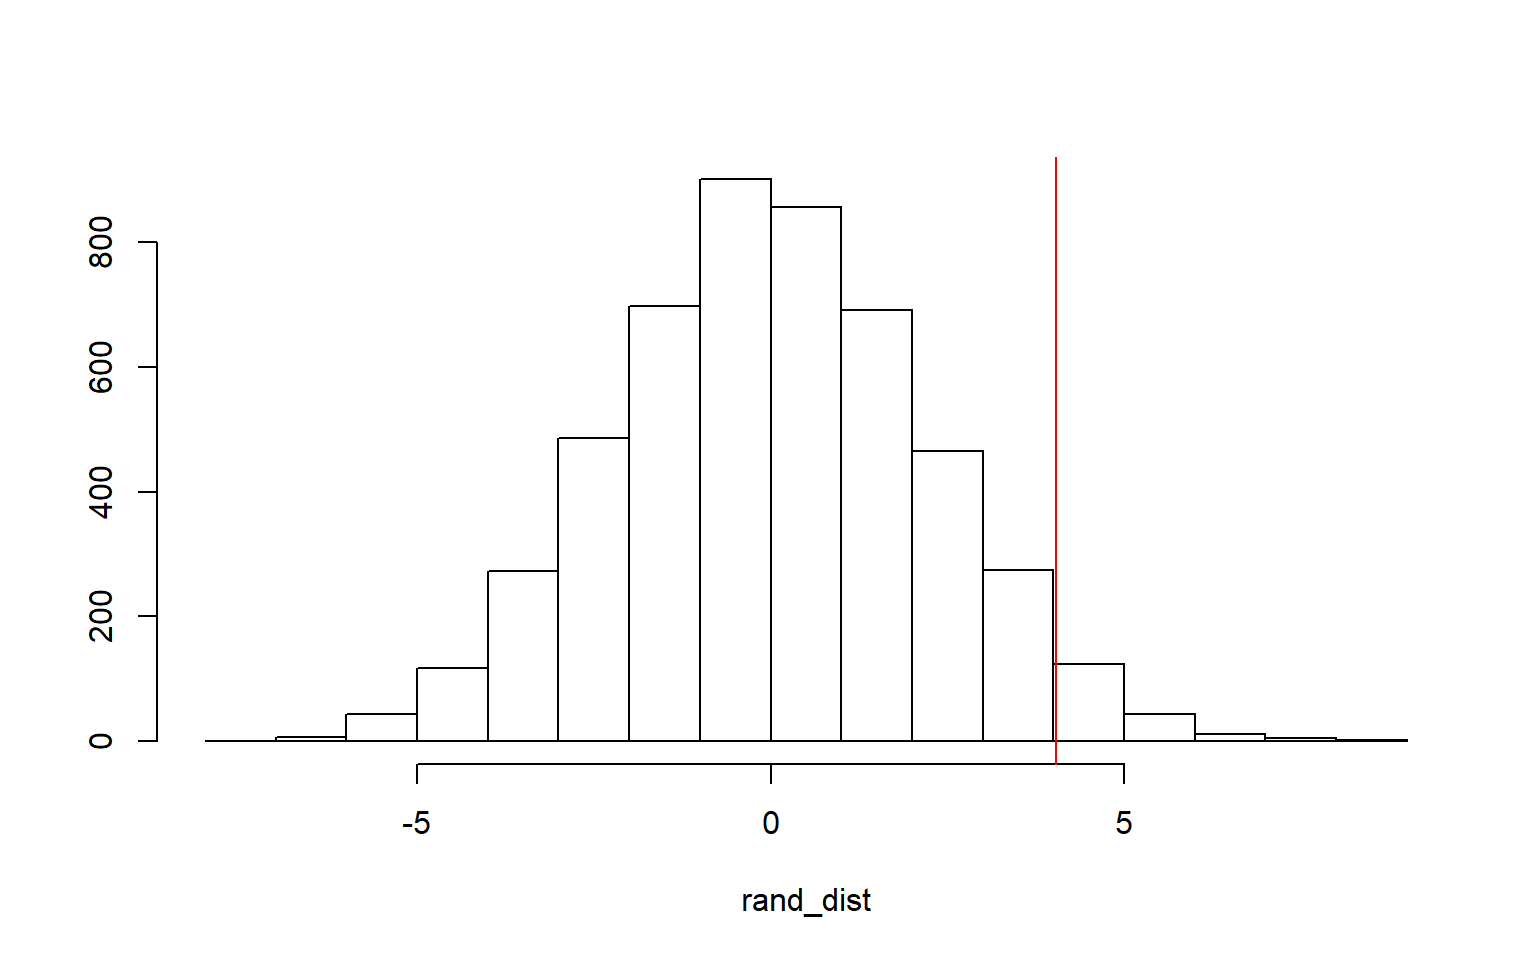
\includegraphics{Project2_files/figure-latex/unnamed-chunk-3-1} \end{center}

\begin{Shaded}
\begin{Highlighting}[]
\KeywordTok{mean}\NormalTok{(rand_dist}\OperatorTok{>}\FloatTok{4.037338}\NormalTok{)}\OperatorTok{*}\DecValTok{2}
\end{Highlighting}
\end{Shaded}

\begin{verbatim}
## [1] 0.074
\end{verbatim}

\begin{Shaded}
\begin{Highlighting}[]
\KeywordTok{t.test}\NormalTok{(}\DataTypeTok{data=}\NormalTok{dataset1, bdi.pre}\OperatorTok{~}\NormalTok{drug)}
\end{Highlighting}
\end{Shaded}

\begin{verbatim}
##
## Welch Two Sample t-test
##
## data: bdi.pre by drug
## t = -1.7995, df = 74.911, p-value = 0.07597
## alternative hypothesis: true difference in means is not
equal to 0
## 95 percent confidence interval:
## -8.5069019 0.4322266
## sample estimates:
## mean in group No mean in group Yes
## 21.55357 25.59091
\end{verbatim}

\emph{The Null Hypothesis is that the mean starting Beck Depression
Inventory II score is the same for patients on vs patients off
anti-depressents. The Alternative Hypothesis is that the mean starting
Beck Depression Inventory II score is different for patients on verus
off anti depressents. After generating a distribution of 5000 mean
differnces via a randomization test, the p value was 0.0644 which is
larger than 0.05. Thus, we can refuse to reject the null hypothesis and
say that there is not a signifcant difference in the pre-treatment Beck
Depression Inventory score for patients on versus off anti-depressents;
the independet t test for compariosn confimred this interpretation.}

\emph{Build a linear regression model predicting one of your response
variables from at least 2 other variables, including their interaction.
Mean-center any numeric variables involved in the inter- action.}

\begin{Shaded}
\begin{Highlighting}[]
\KeywordTok{library}\NormalTok{(lmtest)}
\KeywordTok{library}\NormalTok{(sandwich)}
\KeywordTok{library}\NormalTok{(tidyverse)}
\KeywordTok{library}\NormalTok{(dplyr)}

\NormalTok{dataset1}\OperatorTok{$}\NormalTok{bdi}\FloatTok{.8}\NormalTok{m_c1 <-dataset1}\OperatorTok{$}\NormalTok{bdi}\FloatTok{.8}\NormalTok{m}\OperatorTok{-}\KeywordTok{mean}\NormalTok{(dataset1}\OperatorTok{$}\NormalTok{bdi}\FloatTok{.8}\NormalTok{m,}\DataTypeTok{na.rm=}\OtherTok{TRUE}\NormalTok{)}

\NormalTok{dataset1}\OperatorTok{$}\NormalTok{bdi.pre_c1 <-dataset1}\OperatorTok{$}\NormalTok{bdi.pre}\OperatorTok{-}\KeywordTok{mean}\NormalTok{(dataset1}\OperatorTok{$}\NormalTok{bdi.pre,}\DataTypeTok{na.rm=}\OtherTok{TRUE}\NormalTok{)}

\NormalTok{fit <-}\KeywordTok{lm}\NormalTok{(bdi}\FloatTok{.8}\NormalTok{m_c1 }\OperatorTok{~}\StringTok{ }\NormalTok{treatment }\OperatorTok{*}\StringTok{ }\NormalTok{bdi.pre_c1, }\DataTypeTok{data=}\NormalTok{dataset1)}
\KeywordTok{summary}\NormalTok{(fit)}
\end{Highlighting}
\end{Shaded}

\begin{verbatim}
##
## Call:
## lm(formula = bdi.8m_c1 ~ treatment * bdi.pre_c1, data =
dataset1)
##
## Residuals:
## Min 1Q Median 3Q Max
## -18.8875 -5.3813 0.0658 3.7307 19.5346
##
## Coefficients:
## Estimate Std. Error t value Pr(>|t|)
## (Intercept) 2.0088 1.7005 1.181 0.2433
## treatmentBtheB -3.9839 2.3630 -1.686 0.0983 .
## bdi.pre_c1 0.5779 0.2139 2.702 0.0095 **
## treatmentBtheB:bdi.pre_c1 -0.3465 0.2626 -1.320 0.1932
## ---
## Signif. codes: 0 '***' 0.001 '**' 0.01 '*' 0.05 '.' 0.1
' ' 1
##
## Residual standard error: 8.46 on 48 degrees of freedom
## (48 observations deleted due to missingness)
## Multiple R-squared: 0.222, Adjusted R-squared: 0.1734
## F-statistic: 4.566 on 3 and 48 DF, p-value: 0.006818
\end{verbatim}

\begin{Shaded}
\begin{Highlighting}[]
\NormalTok{dataset1}\OperatorTok\KeywordTok{ggplot}\NormalTok{(}\KeywordTok{aes}\NormalTok{(}\DataTypeTok{x=}\NormalTok{bdi}\FloatTok{.8}\NormalTok{m_c1, }\DataTypeTok{y=}\NormalTok{treatment, }\DataTypeTok{color=}\NormalTok{bdi.pre)) }\OperatorTok{+}\StringTok{ }\KeywordTok{geom_point}\NormalTok{()}\OperatorTok{+}\KeywordTok{geom_line}\NormalTok{()}
\end{Highlighting}
\end{Shaded}

\begin{center}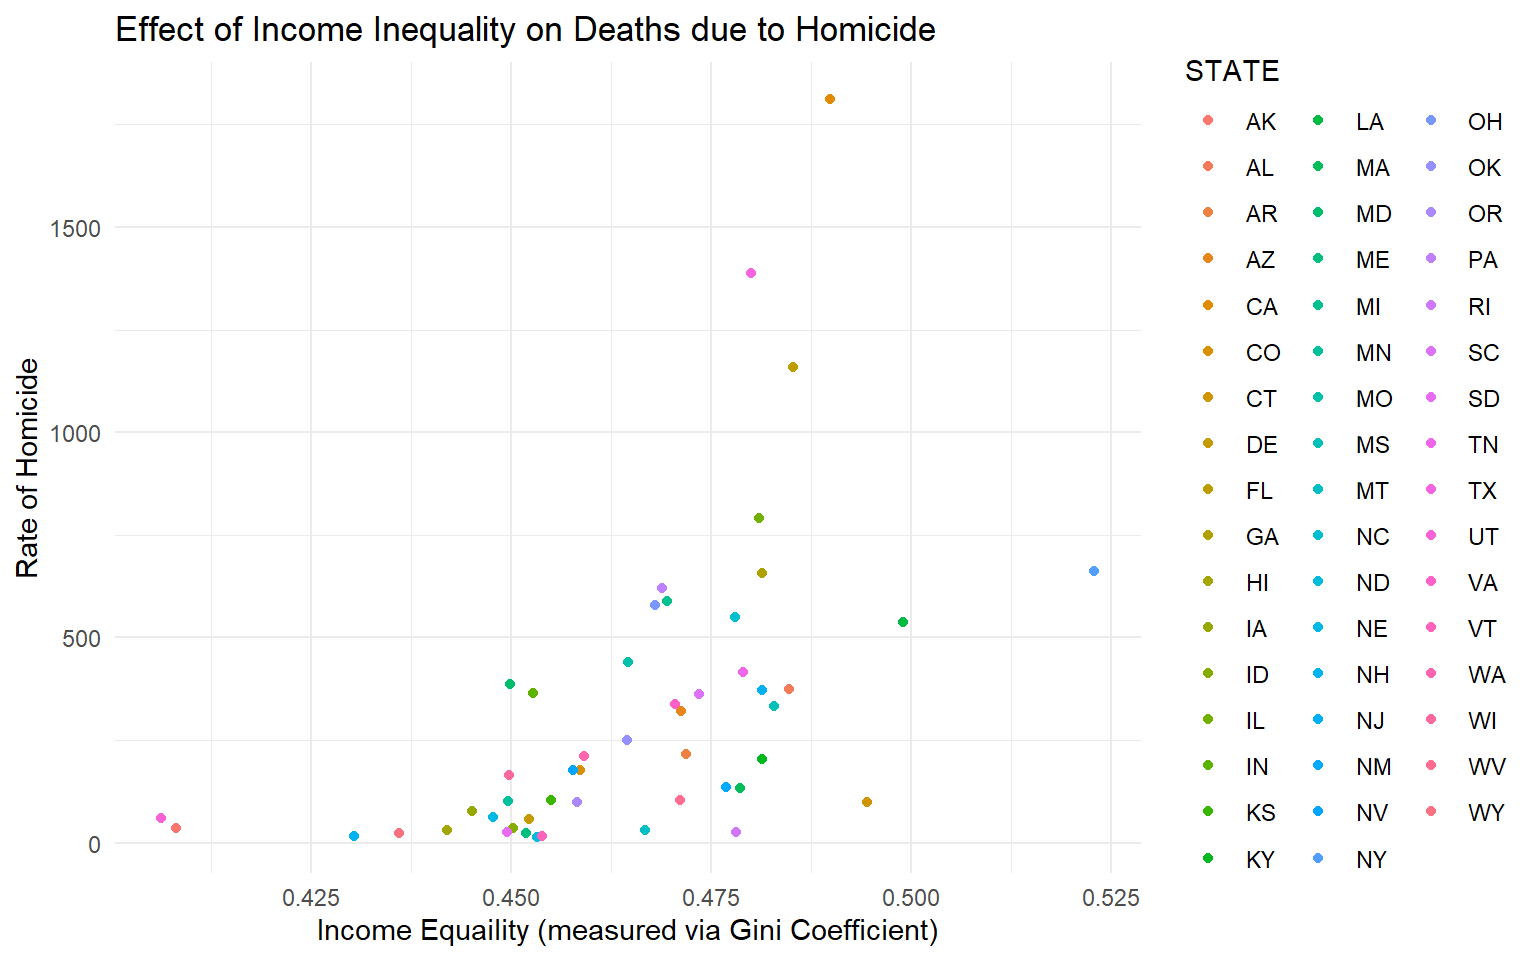
\includegraphics{Project2_files/figure-latex/unnamed-chunk-4-1} \end{center}

\begin{Shaded}
\begin{Highlighting}[]
\KeywordTok{bptest}\NormalTok{(fit)}\CommentTok{#0.008}
\end{Highlighting}
\end{Shaded}

\begin{verbatim}
## 
##  studentized Breusch-Pagan test
## 
## data:  fit
## BP = 11.831, df = 3, p-value = 0.007985
\end{verbatim}

\begin{Shaded}
\begin{Highlighting}[]
\NormalTok{resids<-fit}\OperatorTok{$}\NormalTok{residuals}
\NormalTok{fitvals<-fit}\OperatorTok{$}\NormalTok{fitted.values}
\KeywordTok{ggplot}\NormalTok{()}\OperatorTok{+}\KeywordTok{geom_point}\NormalTok{(}\KeywordTok{aes}\NormalTok{(fitvals,resids))}\OperatorTok{+}\KeywordTok{geom_hline}\NormalTok{(}\DataTypeTok{yintercept=}\DecValTok{0}\NormalTok{, }\DataTypeTok{color=}\StringTok{'red'}\NormalTok{)}
\end{Highlighting}
\end{Shaded}

\begin{center}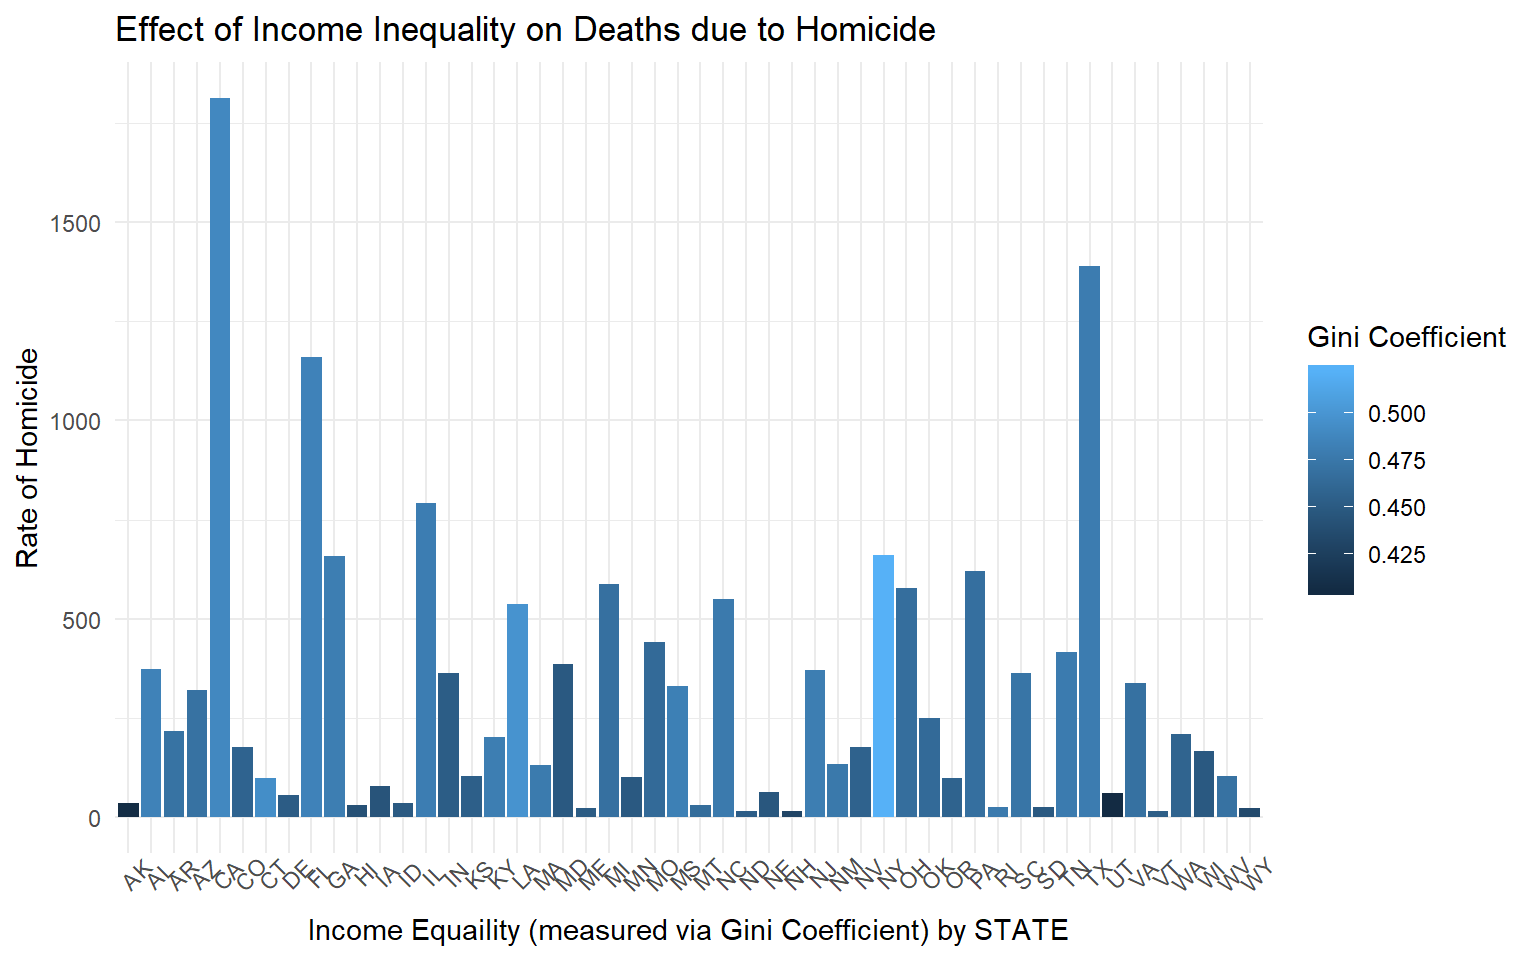
\includegraphics{Project2_files/figure-latex/unnamed-chunk-4-2} \end{center}

\begin{Shaded}
\begin{Highlighting}[]
\KeywordTok{shapiro.test}\NormalTok{(resids)}\CommentTok{#0.8238}
\end{Highlighting}
\end{Shaded}

\begin{verbatim}
## 
##  Shapiro-Wilk normality test
## 
## data:  resids
## W = 0.98666, p-value = 0.8238
\end{verbatim}

\begin{Shaded}
\begin{Highlighting}[]
\KeywordTok{coeftest}\NormalTok{(fit,}\DataTypeTok{vcov=}\KeywordTok{vcovHC}\NormalTok{(fit))}
\end{Highlighting}
\end{Shaded}

\begin{verbatim}
##
## t test of coefficients:
##
## Estimate Std. Error t value Pr(>|t|)
## (Intercept) 2.00885 2.20444 0.9113 0.3667
## treatmentBtheB -3.98389 2.49231 -1.5985 0.1165
## bdi.pre_c1 0.57790 0.33835 1.7080 0.0941 .
## treatmentBtheB:bdi.pre_c1 -0.34653 0.35556 -0.9746
0.3346
## ---
## Signif. codes: 0 '***' 0.001 '**' 0.01 '*' 0.05 '.' 0.1
' ' 1
\end{verbatim}

\begin{Shaded}
\begin{Highlighting}[]
\KeywordTok{summary}\NormalTok{(fit)}\OperatorTok{$}\NormalTok{r.sq}
\end{Highlighting}
\end{Shaded}

\begin{verbatim}
## [1] 0.2220036
\end{verbatim}

\emph{Based on regression results, when no treatment is applied and the
``bdi.pre'' (starting Beck Depression Inventory II Score) is zero, the
Beck Depression Inventory II Score after 8 months of treatment is
2.0088. On average, for every 1 unit increase in the Beat the Blues
treatment, the Beck Depression Inventory II Score after 8 months of
treatment decreases by about 3.9839 units. For every one unit increase
in `bdi.pre', on average, the Beck Depression Inventory II Score after 8
months of treatment increases by about 0.5779 units. On average, for
every one unit increase in the interaction between treatment and
pre-treatment Beck Depression Inventory II Score, the Beck Depression
Inventory II Score after 8 months of Beat the Blues treatment decreases
by -0.3465. When looking at the assumptions, it failed to meet the
homsckedasticty assumption as the Breusch-Pagan test returned a p-value
less than 0.05 so the null hypothesis of homescadaskcity was accepted.
Contrastly, it met the normality assumption as after performing the
Shapiro-Wilk test p-value was greater than 0.05 so I failed to reject
the null hypothesis of normality. Lastly, through looking at the coded
graph it met the linearity assumption as all the lines were straight.
When comparing robust SE and original SE, the robust SE increased for
all the coeffients. The treatment Beat the Blues, the interaction
between Beat the Blues and pre-treatment bdi score, and the
pre-treatment bdi score had no signigcnat effect on the patients Beck
Depression Inventory Score 8 months after treatment as the p-value were
less than 0.05 (0.1165 and 0.3346 respectively). However, before
computing the roboust SE, the p-value of bdi.pre was 0.0095 (less than
0.05) and thus had a signifcant effect on Beck Depression INventory
Score after 8 months. Overall, my model explains 22.20\% of the
variation in the outcome. } *

\emph{(5 pts) Rerun same regression model (with interaction), but this
time compute bootstrapped standard errors. Discuss any changes you
observe in SEs and p-values using these SEs compared to the original SEs
and the robust SEs)}

\begin{Shaded}
\begin{Highlighting}[]
\NormalTok{samp_distn<-}\KeywordTok{replicate}\NormalTok{(}\DecValTok{5000}\NormalTok{, \{}
\NormalTok{  boot_data<-dataset1[}\KeywordTok{sample}\NormalTok{(}\KeywordTok{nrow}\NormalTok{(dataset1),}\DataTypeTok{replace=}\OtherTok{TRUE}\NormalTok{),]}
\NormalTok{  fit1<-}\KeywordTok{lm}\NormalTok{(bdi}\FloatTok{.8}\NormalTok{m_c1}\OperatorTok{~}\NormalTok{treatment}\OperatorTok{*}\NormalTok{bdi.pre_c1,}\DataTypeTok{data=}\NormalTok{boot_data)}
  \KeywordTok{coef}\NormalTok{(fit1)}
\NormalTok{\})}
\CommentTok{## Estimated SEs}
\NormalTok{samp_distn}\OperatorTok\NormalTok{t}\OperatorTok\NormalTok{as.data.frame}\OperatorTok\KeywordTok{summarize_all}\NormalTok{(sd)}
\end{Highlighting}
\end{Shaded}

\begin{verbatim}
## (Intercept) treatmentBtheB bdi.pre_c1
treatmentBtheB:bdi.pre_c1
## 1 2.066198 2.364539 0.317116 0.3371881
\end{verbatim}

\emph{The Bootstrapped SE are less than the roboust SE for all variables
and greater than all the original SE as well except for Treatment which
is slightly lower.}

\begin{itemize}
\tightlist
\item
  Perform a logistic regression predicting a binary categorical variable
  (if you don't have one, make/get one) from at least two explanatory
  variables (interaction not necessary)*
\end{itemize}

\begin{Shaded}
\begin{Highlighting}[]
\NormalTok{dataset1}\OperatorTok{$}\NormalTok{y<-}\KeywordTok{ifelse}\NormalTok{(dataset1}\OperatorTok{$}\NormalTok{drug}\OperatorTok{==}\StringTok{'Yes'}\NormalTok{,}\DecValTok{1}\NormalTok{,}\DecValTok{0}\NormalTok{)}
\NormalTok{fit3<-}\KeywordTok{glm}\NormalTok{(drug}\OperatorTok{~}\NormalTok{treatment}\OperatorTok{+}\NormalTok{length,}\DataTypeTok{data=}\NormalTok{dataset1,}\DataTypeTok{family=}\KeywordTok{binomial}\NormalTok{(}\DataTypeTok{link=}\StringTok{"logit"}\NormalTok{))}
\KeywordTok{coeftest}\NormalTok{(fit3)}
\end{Highlighting}
\end{Shaded}

\begin{verbatim}
##
## z test of coefficients:
##
## Estimate Std. Error z value Pr(>|z|)
## (Intercept) -0.59956 0.37542 -1.5970 0.110258
## treatmentBtheB 1.20978 0.42874 2.8217 0.004776 **
## length>6m -0.58680 0.42560 -1.3788 0.167964
## ---
## Signif. codes: 0 '***' 0.001 '**' 0.01 '*' 0.05 '.' 0.1
' ' 1
\end{verbatim}

\begin{Shaded}
\begin{Highlighting}[]
\KeywordTok{exp}\NormalTok{(}\KeywordTok{coef}\NormalTok{(fit3))}
\end{Highlighting}
\end{Shaded}

\begin{verbatim}
##    (Intercept) treatmentBtheB      length>6m 
##      0.5490540      3.3527448      0.5561039
\end{verbatim}

\begin{Shaded}
\begin{Highlighting}[]
\NormalTok{dataset1}\OperatorTok{$}\NormalTok{probability <-}\KeywordTok{predict}\NormalTok{(fit3, }\DataTypeTok{data=}\NormalTok{dataset1, }\DataTypeTok{type =} \StringTok{"response"}\NormalTok{)}
\KeywordTok{table}\NormalTok{(}\DataTypeTok{predict=}\KeywordTok{as.numeric}\NormalTok{(dataset1}\OperatorTok{$}\NormalTok{probability}\OperatorTok{>}\NormalTok{.}\DecValTok{5}\NormalTok{),}\DataTypeTok{truth=}\NormalTok{dataset1}\OperatorTok{$}\NormalTok{y)}\OperatorTok\NormalTok{addmargins}
\end{Highlighting}
\end{Shaded}

\begin{verbatim}
##        truth
## predict   0   1 Sum
##     0    34  14  48
##     1    22  30  52
##     Sum  56  44 100
\end{verbatim}

\begin{Shaded}
\begin{Highlighting}[]
\NormalTok{Accurancy <-(}\DecValTok{34}\OperatorTok{+}\DecValTok{30}\NormalTok{)}\OperatorTok{/}\DecValTok{100}
\NormalTok{TPR <-}\StringTok{ }\DecValTok{30}\OperatorTok{/}\DecValTok{44}
\NormalTok{TNR<-}\StringTok{ }\DecValTok{34}\OperatorTok{/}\DecValTok{56}
\NormalTok{PVR<-}\DecValTok{30}\OperatorTok{/}\DecValTok{52}

\KeywordTok{mean}\NormalTok{(dataset1[dataset1}\OperatorTok{$}\NormalTok{y}\OperatorTok{==}\DecValTok{1}\NormalTok{,]}\OperatorTok{$}\NormalTok{probability}\OperatorTok{>}\NormalTok{.}\DecValTok{5}\NormalTok{)}
\end{Highlighting}
\end{Shaded}

\begin{verbatim}
## [1] 0.6818182
\end{verbatim}

\begin{Shaded}
\begin{Highlighting}[]
\KeywordTok{ggplot}\NormalTok{(dataset1)}\OperatorTok{+}\KeywordTok{aes}\NormalTok{(probability, drug)}\OperatorTok{+}\KeywordTok{geom_line}\NormalTok{()}
\end{Highlighting}
\end{Shaded}

\begin{center}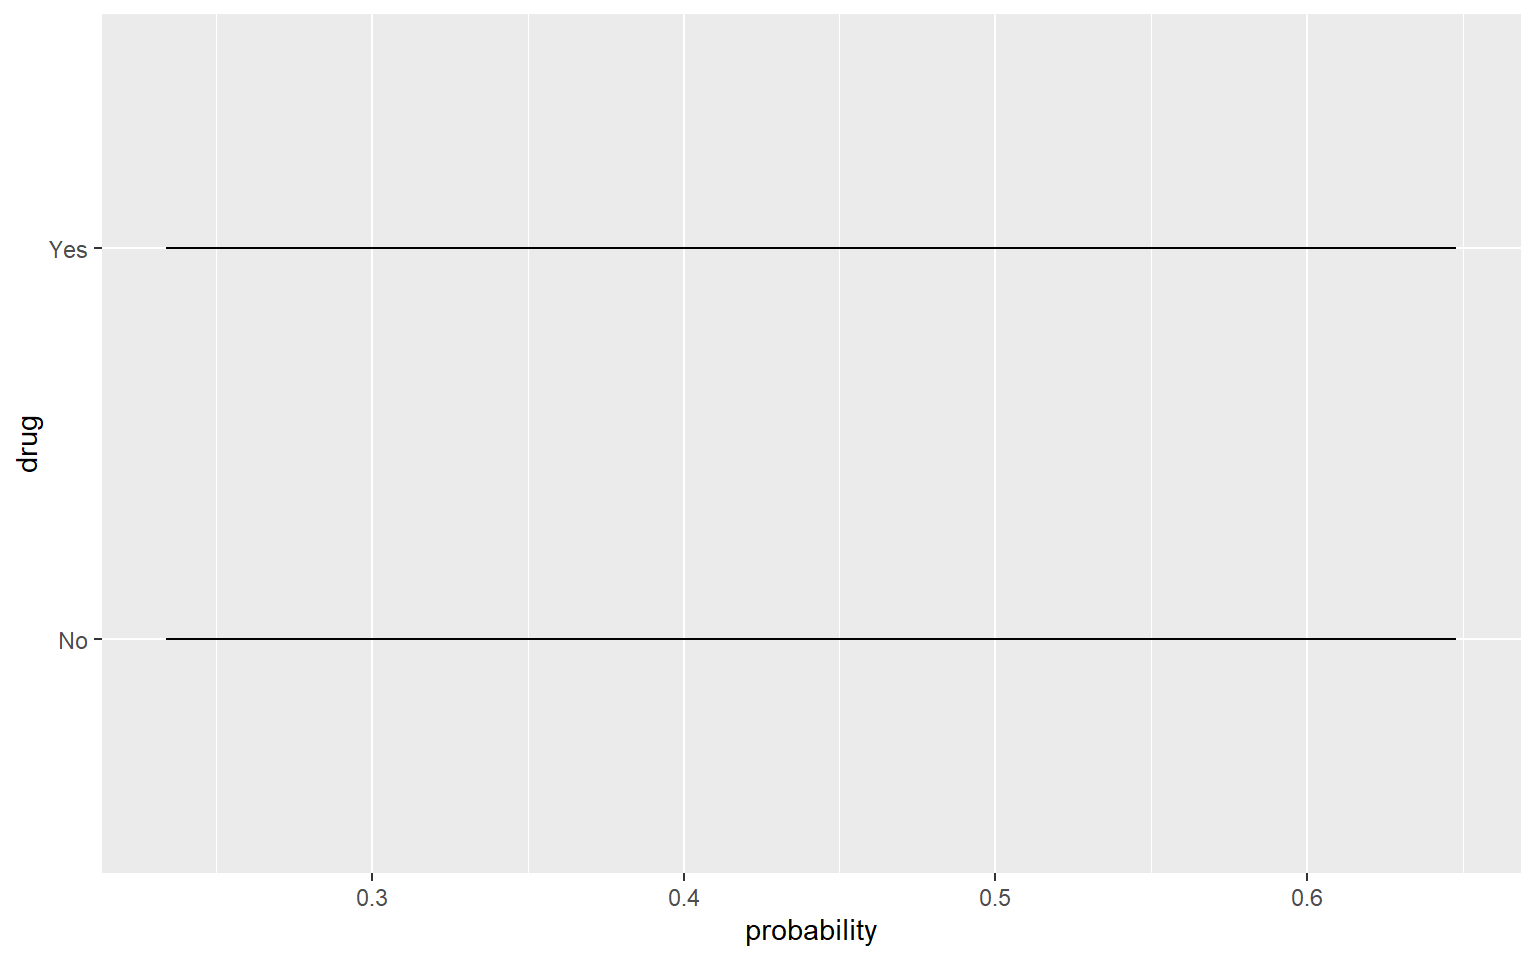
\includegraphics{Project2_files/figure-latex/unnamed-chunk-6-1} \end{center}

\begin{Shaded}
\begin{Highlighting}[]
\KeywordTok{library}\NormalTok{(plotROC)}
\NormalTok{ROCplot<-}\KeywordTok{ggplot}\NormalTok{(dataset1)}\OperatorTok{+}\KeywordTok{geom_roc}\NormalTok{(}\KeywordTok{aes}\NormalTok{(}\DataTypeTok{d=}\NormalTok{y,}\DataTypeTok{m=}\NormalTok{probability), }\DataTypeTok{n.cuts=}\DecValTok{0}\NormalTok{)}\OperatorTok{+}
\KeywordTok{geom_segment}\NormalTok{(}\KeywordTok{aes}\NormalTok{(}\DataTypeTok{x=}\DecValTok{0}\NormalTok{,}\DataTypeTok{xend=}\DecValTok{1}\NormalTok{,}\DataTypeTok{y=}\DecValTok{0}\NormalTok{,}\DataTypeTok{yend=}\DecValTok{1}\NormalTok{),}\DataTypeTok{lty=}\DecValTok{2}\NormalTok{)}
\NormalTok{ROCplot}
\end{Highlighting}
\end{Shaded}

\begin{center}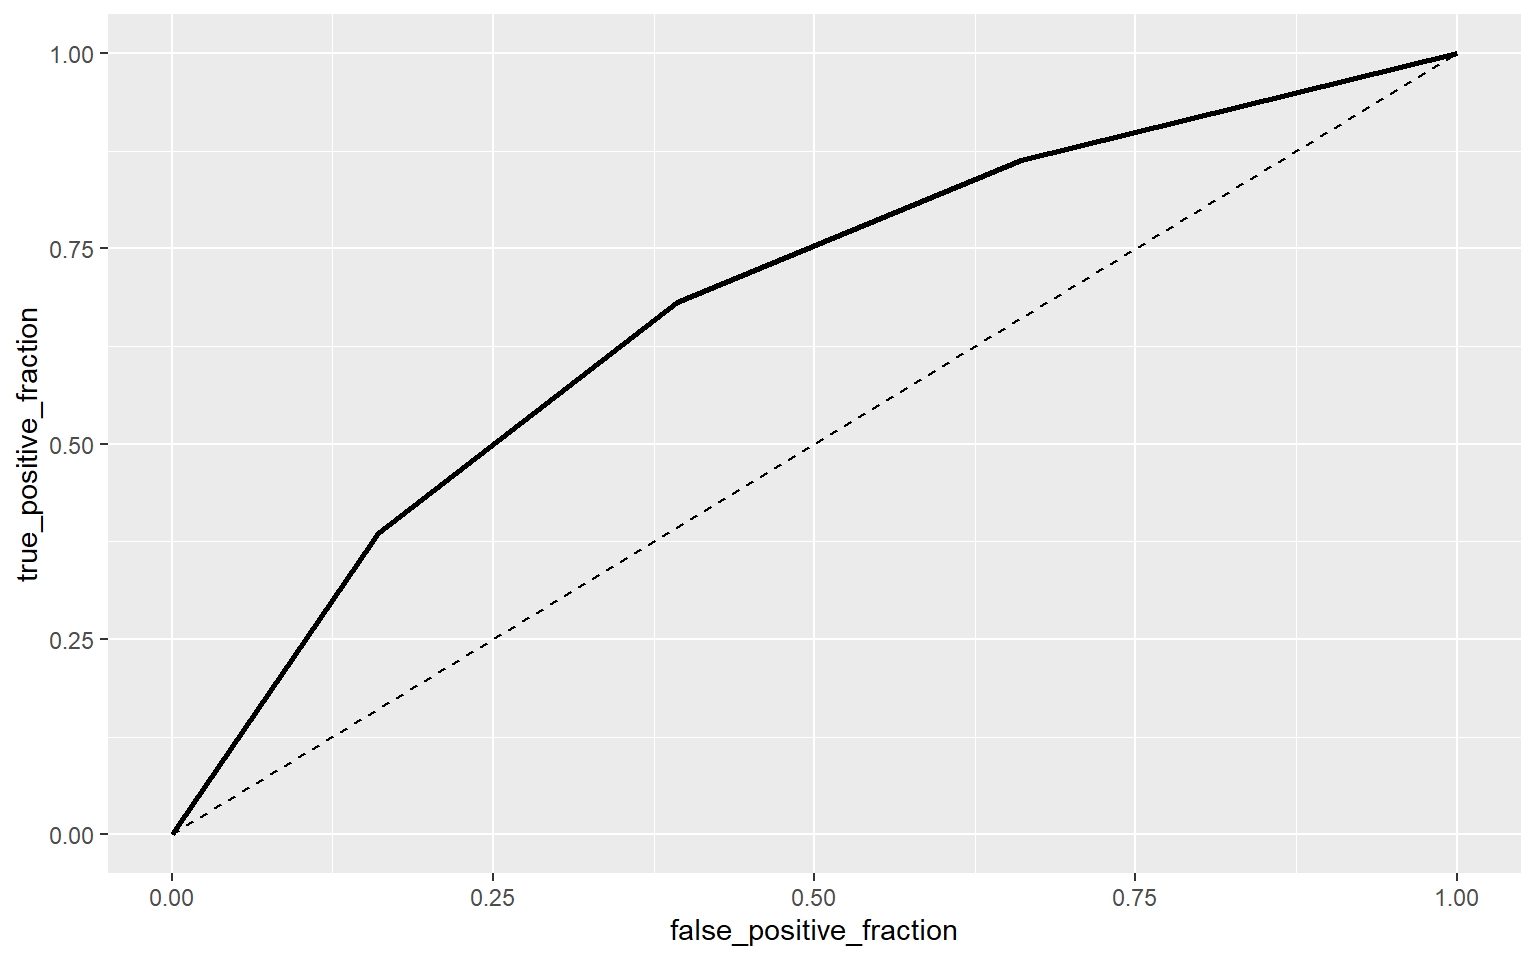
\includegraphics{Project2_files/figure-latex/unnamed-chunk-6-2} \end{center}

\begin{Shaded}
\begin{Highlighting}[]
\KeywordTok{calc_auc}\NormalTok{(ROCplot)}
\end{Highlighting}
\end{Shaded}

\begin{verbatim}
##   PANEL group       AUC
## 1     1    -1 0.6781656
\end{verbatim}

\begin{Shaded}
\begin{Highlighting}[]
\NormalTok{class_diag<-}\ControlFlowTok{function}\NormalTok{(probs,truth)\{}
\NormalTok{ tab<-}\KeywordTok{table}\NormalTok{(}\KeywordTok{factor}\NormalTok{(probs}\OperatorTok{>}\NormalTok{.}\DecValTok{5}\NormalTok{,}\DataTypeTok{levels=}\KeywordTok{c}\NormalTok{(}\StringTok{"FALSE"}\NormalTok{,}\StringTok{"TRUE"}\NormalTok{)),truth)}
\NormalTok{ acc=}\KeywordTok{sum}\NormalTok{(}\KeywordTok{diag}\NormalTok{(tab))}\OperatorTok{/}\KeywordTok{sum}\NormalTok{(tab)}
\NormalTok{ sens=tab[}\DecValTok{2}\NormalTok{,}\DecValTok{2}\NormalTok{]}\OperatorTok{/}\KeywordTok{colSums}\NormalTok{(tab)[}\DecValTok{2}\NormalTok{]}
\NormalTok{ spec=tab[}\DecValTok{1}\NormalTok{,}\DecValTok{1}\NormalTok{]}\OperatorTok{/}\KeywordTok{colSums}\NormalTok{(tab)[}\DecValTok{1}\NormalTok{]}
\NormalTok{ ppv=tab[}\DecValTok{2}\NormalTok{,}\DecValTok{2}\NormalTok{]}\OperatorTok{/}\KeywordTok{rowSums}\NormalTok{(tab)[}\DecValTok{2}\NormalTok{]}
 \ControlFlowTok{if}\NormalTok{(}\KeywordTok{is.numeric}\NormalTok{(truth)}\OperatorTok{==}\OtherTok{FALSE} \OperatorTok{&}\StringTok{ }\KeywordTok{is.logical}\NormalTok{(truth)}\OperatorTok{==}\OtherTok{FALSE}\NormalTok{) truth<-}\KeywordTok{as.numeric}\NormalTok{(truth)}\OperatorTok{-}\DecValTok{1}
 \CommentTok{#CALCULATE EXACT AUC}
\NormalTok{ ord<-}\KeywordTok{order}\NormalTok{(probs, }\DataTypeTok{decreasing=}\OtherTok{TRUE}\NormalTok{)}
\NormalTok{ probs <-}\StringTok{ }\NormalTok{probs[ord]; truth <-}\StringTok{ }\NormalTok{truth[ord]}
\NormalTok{ TPR=}\KeywordTok{cumsum}\NormalTok{(truth)}\OperatorTok{/}\KeywordTok{max}\NormalTok{(}\DecValTok{1}\NormalTok{,}\KeywordTok{sum}\NormalTok{(truth))}
\NormalTok{ FPR=}\KeywordTok{cumsum}\NormalTok{(}\OperatorTok{!}\NormalTok{truth)}\OperatorTok{/}\KeywordTok{max}\NormalTok{(}\DecValTok{1}\NormalTok{,}\KeywordTok{sum}\NormalTok{(}\OperatorTok{!}\NormalTok{truth))}
\NormalTok{ dup<-}\KeywordTok{c}\NormalTok{(probs[}\OperatorTok{-}\DecValTok{1}\NormalTok{]}\OperatorTok{>=}\NormalTok{probs[}\OperatorTok{-}\KeywordTok{length}\NormalTok{(probs)], }\OtherTok{FALSE}\NormalTok{)}
\NormalTok{ TPR<-}\KeywordTok{c}\NormalTok{(}\DecValTok{0}\NormalTok{,TPR[}\OperatorTok{!}\NormalTok{dup],}\DecValTok{1}\NormalTok{); FPR<-}\KeywordTok{c}\NormalTok{(}\DecValTok{0}\NormalTok{,FPR[}\OperatorTok{!}\NormalTok{dup],}\DecValTok{1}\NormalTok{)}
\NormalTok{ n <-}\StringTok{ }\KeywordTok{length}\NormalTok{(TPR)}
\NormalTok{ auc<-}\StringTok{ }\KeywordTok{sum}\NormalTok{( ((TPR[}\OperatorTok{-}\DecValTok{1}\NormalTok{]}\OperatorTok{+}\NormalTok{TPR[}\OperatorTok{-}\NormalTok{n])}\OperatorTok{/}\DecValTok{2}\NormalTok{) }\OperatorTok{*}\StringTok{ }\NormalTok{(FPR[}\OperatorTok{-}\DecValTok{1}\NormalTok{]}\OperatorTok{-}\NormalTok{FPR[}\OperatorTok{-}\NormalTok{n]) )}
 \KeywordTok{data.frame}\NormalTok{(acc,sens,spec,ppv,auc)}
\NormalTok{\} }

\KeywordTok{set.seed}\NormalTok{(}\DecValTok{1234}\NormalTok{)}
\NormalTok{k=}\DecValTok{10} 
\NormalTok{data1<-dataset1[}\KeywordTok{sample}\NormalTok{(}\KeywordTok{nrow}\NormalTok{(dataset1)),] }
\NormalTok{folds<-}\KeywordTok{cut}\NormalTok{(}\KeywordTok{seq}\NormalTok{(}\DecValTok{1}\OperatorTok{:}\KeywordTok{nrow}\NormalTok{(dataset1)),}\DataTypeTok{breaks=}\NormalTok{k,}\DataTypeTok{labels=}\NormalTok{F) }
\NormalTok{diags<-}\OtherTok{NULL}
\ControlFlowTok{for}\NormalTok{(i }\ControlFlowTok{in} \DecValTok{1}\OperatorTok{:}\NormalTok{k)\{}
 
\NormalTok{ train<-data1[folds}\OperatorTok{!=}\NormalTok{i,]}
\NormalTok{ test<-data1[folds}\OperatorTok{==}\NormalTok{i,]}
\NormalTok{ truth<-test}\OperatorTok{$}\NormalTok{y}
 
\NormalTok{ fit5<-}\KeywordTok{glm}\NormalTok{(y}\OperatorTok{~}\NormalTok{treatment}\OperatorTok{+}\NormalTok{bdi.pre_c1,}\DataTypeTok{data=}\NormalTok{train,}\DataTypeTok{family=}\StringTok{"binomial"}\NormalTok{)}
\NormalTok{ probs<-}\KeywordTok{predict}\NormalTok{(fit5,}\DataTypeTok{newdata =}\NormalTok{ test,}\DataTypeTok{type=}\StringTok{"response"}\NormalTok{)}
 
\NormalTok{ diags<-}\KeywordTok{rbind}\NormalTok{(diags,}\KeywordTok{class_diag}\NormalTok{(probs,truth))}
\NormalTok{\}}

\KeywordTok{apply}\NormalTok{(diags,}\DecValTok{2}\NormalTok{,mean)}
\end{Highlighting}
\end{Shaded}

\begin{verbatim}
##       acc      sens      spec       ppv       auc 
## 0.6400000 0.5666667 0.7386905 0.6516667 0.7163690
\end{verbatim}

\emph{When no treatment is applied and the length of the depressive
episode is 0 months, the odds of the patients having used
anti-depressents is 0.5491. When the length of the depressive episode is
held constant, for every one unit increase in the Beat the Blues
treatment, the odds of the pateint having taken anti-depressents
increases by 3.353. When the application of treatment is held constant,
for every 1 month increases in the length of the depressive episode, the
odds of the patient having used anti-depressents increases by 0.5561.
The Accuracy (the proportion of correctly classified cases) was 0.64,
the Sensitivity (True Positive Rate, TPR) which is proportion of
patients using drugs (1 cases) coreectly classified was 0.681,
Specficity which is the proportion of pateints not using drugs (``0
cases'') correctly classified was 0.607.Precsion (Positive Predictive
Value, PPV) proportion classified as using drugs who actaully use drugs
was 0.5769. The AUC was 0.6781which is the probability that a randomly
selected person taking drugs has a higher prediction than a randomly
selected person not taking drugs. Overall, with it being 0.681 length of
depressive episode and pre-treatment BDI are moderate preictors of a
pateints taking anti-depressents. After the 10 Fold CV, the accurancy
was 0.60, the senstivity was 0.4433, the specficity was 0.6957, the ppv
was 0.60, and the auc was 0.6747.}

\begin{enumerate}
\def\labelenumi{\arabic{enumi})}
\setcounter{enumi}{5}
\item
\end{enumerate}

\begin{Shaded}
\begin{Highlighting}[]
\KeywordTok{library}\NormalTok{(glmnet)}



\NormalTok{fit50<-}\KeywordTok{glm}\NormalTok{(bdi}\FloatTok{.8}\NormalTok{m}\OperatorTok{~}\StringTok{ }\DecValTok{-1} \OperatorTok{+}\StringTok{ }\KeywordTok{as.factor}\NormalTok{(length)}\OperatorTok{+}\KeywordTok{as.factor}\NormalTok{(treatment)}\OperatorTok{+}\KeywordTok{as.factor}\NormalTok{(drug)}\OperatorTok{+}\NormalTok{bdi.pre, }\DataTypeTok{data =}\NormalTok{ dataset1)}
\KeywordTok{model.matrix}\NormalTok{(fit)}
\end{Highlighting}
\end{Shaded}

\begin{verbatim}
## (Intercept) treatmentBtheB bdi.pre_c1
treatmentBtheB:bdi.pre_c1
## 2 1 1 8.67 8.67
## 4 1 1 -2.33 -2.33
## 6 1 1 -16.33 -16.33
## 7 1 0 -6.33 0.00
## 8 1 0 -3.33 0.00
## 9 1 1 -5.33 -5.33
## 10 1 1 -3.33 -3.33
## 11 1 0 6.67 0.00
## 14 1 0 6.67 0.00
## 15 1 1 -0.33 -0.33
## 16 1 0 -7.33 0.00
## 18 1 1 -10.33 -10.33
## 19 1 0 13.67 0.00
## 20 1 1 11.67 11.67
## 22 1 0 2.67 0.00
## 29 1 1 12.67 12.67
## 30 1 1 -13.33 -13.33
## 31 1 0 3.67 0.00
## 32 1 1 -5.33 -5.33
## 33 1 1 -12.33 -12.33
## 35 1 1 20.67 20.67
## 37 1 0 -2.33 0.00
## 38 1 0 10.67 0.00
## 40 1 0 14.67 0.00
## 42 1 0 -3.33 0.00
## 43 1 0 -6.33 0.00
## 45 1 1 18.67 18.67
## 47 1 1 9.67 9.67
## 50 1 0 12.67 0.00
## 53 1 0 7.67 0.00
## 56 1 1 -16.33 -16.33
## 61 1 0 -1.33 0.00
## 62 1 0 -0.33 0.00
## 67 1 0 -6.33 0.00
## 71 1 1 -14.33 -14.33
## 75 1 0 -9.33 0.00
## 76 1 1 4.67 4.67
## 77 1 1 -8.33 -8.33
## 78 1 1 -1.33 -1.33
## 80 1 0 -2.33 0.00
## 81 1 0 3.67 0.00
## 83 1 0 -13.33 0.00
## 84 1 0 -2.33 0.00
## 86 1 1 12.67 12.67
## 88 1 0 11.67 0.00
## 89 1 1 9.67 9.67
## 90 1 1 -4.33 -4.33
## 94 1 1 -4.33 -4.33
## 95 1 1 -7.33 -7.33
## 96 1 1 -7.33 -7.33
## 98 1 1 -12.33 -12.33
## 99 1 0 -10.33 0.00
## attr(,"assign")
## [1] 0 1 2 3
## attr(,"contrasts")
## attr(,"contrasts")$treatment
## [1] "contr.treatment"
\end{verbatim}

\begin{Shaded}
\begin{Highlighting}[]
\KeywordTok{set.seed}\NormalTok{(}\DecValTok{1234}\NormalTok{)}
\NormalTok{x<-}\KeywordTok{model.matrix}\NormalTok{(fit50)}
\NormalTok{x<-}\KeywordTok{scale}\NormalTok{(x)}
\NormalTok{y<-}\KeywordTok{as.matrix}\NormalTok{(}\KeywordTok{na.omit}\NormalTok{(dataset1}\OperatorTok{$}\NormalTok{bdi}\FloatTok{.8}\NormalTok{m))}

\NormalTok{cv2<-}\KeywordTok{cv.glmnet}\NormalTok{(x,y)}
\NormalTok{lasso2<-}\KeywordTok{glmnet}\NormalTok{(x,y,}\DataTypeTok{lambda=}\NormalTok{cv2}\OperatorTok{$}\NormalTok{lambda}\FloatTok{.1}\NormalTok{se)}
\KeywordTok{coef}\NormalTok{(cv2)}
\end{Highlighting}
\end{Shaded}

\begin{verbatim}
## 6 x 1 sparse Matrix of class "dgCMatrix"
##                                       1
## (Intercept)                1.113462e+01
## as.factor(length)<6m      -9.653107e-01
## as.factor(length)>6m       5.165502e-16
## as.factor(treatment)BtheB  .           
## as.factor(drug)Yes         .           
## bdi.pre                    9.300352e-02
\end{verbatim}

\begin{Shaded}
\begin{Highlighting}[]
\KeywordTok{set.seed}\NormalTok{(}\DecValTok{1234}\NormalTok{)}
\NormalTok{k=}\DecValTok{10} 
\NormalTok{data2<-dataset1[}\KeywordTok{sample}\NormalTok{(}\KeywordTok{nrow}\NormalTok{(dataset1)),]}

\NormalTok{folds2<-}\KeywordTok{cut}\NormalTok{(}\KeywordTok{seq}\NormalTok{(}\DecValTok{1}\OperatorTok{:}\KeywordTok{nrow}\NormalTok{(dataset1)),}\DataTypeTok{breaks=}\NormalTok{k,}\DataTypeTok{labels=}\NormalTok{F)}
\NormalTok{diags1<-}\OtherTok{NULL}
\ControlFlowTok{for}\NormalTok{(i }\ControlFlowTok{in} \DecValTok{1}\OperatorTok{:}\NormalTok{k)\{}
 
\NormalTok{ train1<-data2[ folds}\OperatorTok{!=}\NormalTok{i,]}
\NormalTok{ test1<-data2[ folds}\OperatorTok{==}\NormalTok{i,]}
\NormalTok{ truth2<-test1}\OperatorTok{$}\NormalTok{bdi}\FloatTok{.8}\NormalTok{m}
 
\NormalTok{ fit60<-}\KeywordTok{glm}\NormalTok{(bdi}\FloatTok{.8}\NormalTok{m}\OperatorTok{~}\KeywordTok{as.factor}\NormalTok{(length)}\OperatorTok{+}\NormalTok{bdi.pre, }\DataTypeTok{data =}\NormalTok{ train1)}
\NormalTok{ probs3<-}\KeywordTok{predict}\NormalTok{(fit60,}\DataTypeTok{newdata =}\NormalTok{ test1,}\DataTypeTok{type=}\StringTok{"response"}\NormalTok{)}

\NormalTok{diags<-}\KeywordTok{mean}\NormalTok{((truth2}\OperatorTok{-}\NormalTok{probs3)}\OperatorTok{^}\DecValTok{2}\NormalTok{)}
\NormalTok{\}}
\KeywordTok{mean}\NormalTok{(diags1)}
\end{Highlighting}
\end{Shaded}

\begin{verbatim}
## [1] NA
\end{verbatim}

\begin{Shaded}
\begin{Highlighting}[]
\KeywordTok{summary}\NormalTok{(fit50)}
\end{Highlighting}
\end{Shaded}

\begin{verbatim}
##
## Call:
## glm(formula = bdi.8m ~ -1 + as.factor(length) +
as.factor(treatment) +
## as.factor(drug) + bdi.pre, data = dataset1)
##
## Deviance Residuals:
## Min 1Q Median 3Q Max
## -16.1579 -3.6418 -0.2671 2.9920 20.3866
##
## Coefficients:
## Estimate Std. Error t value Pr(>|t|)
## as.factor(length)<6m 4.0619 3.3204 1.223 0.2273
## as.factor(length)>6m 10.0763 3.8976 2.585 0.0129 *
## as.factor(treatment)BtheB -3.0815 2.3837 -1.293 0.2024
## as.factor(drug)Yes -2.1906 2.4776 -0.884 0.3811
## bdi.pre 0.2649 0.1355 1.955 0.0565 .
## ---
## Signif. codes: 0 '***' 0.001 '**' 0.01 '*' 0.05 '.' 0.1
' ' 1
##
## (Dispersion parameter for gaussian family taken to be
65.64442)
##
## Null deviance: 10863.0 on 52 degrees of freedom
## Residual deviance: 3085.3 on 47 degrees of freedom
## (48 observations deleted due to missingness)
## AIC: 371.89
##
## Number of Fisher Scoring iterations: 2
\end{verbatim}

\begin{Shaded}
\begin{Highlighting}[]
\KeywordTok{summary}\NormalTok{(fit60)}
\end{Highlighting}
\end{Shaded}

\begin{verbatim}
##
## Call:
## glm(formula = bdi.8m ~ as.factor(length) + bdi.pre, data
= train1)
##
## Deviance Residuals:
## Min 1Q Median 3Q Max
## -15.1827 -4.0920 -0.5375 4.6034 23.5873
##
## Coefficients:
## Estimate Std. Error t value Pr(>|t|)
## (Intercept) 1.9682 2.9148 0.675 0.5030
## as.factor(length)>6m 6.1639 2.4045 2.563 0.0138 *
## bdi.pre 0.2300 0.1235 1.863 0.0690 .
## ---
## Signif. codes: 0 '***' 0.001 '**' 0.01 '*' 0.05 '.' 0.1
' ' 1
##
## (Dispersion parameter for gaussian family taken to be
59.30091)
##
## Null deviance: 3570.0 on 47 degrees of freedom
## Residual deviance: 2668.5 on 45 degrees of freedom
## (42 observations deleted due to missingness)
## AIC: 337.09
##
## Number of Fisher Scoring iterations: 2
\end{verbatim}

\emph{The only variables retained were length and pre.bdi.
Comparatively, the out of sample RMSE was higher than the original.}

\end{document}
